\documentclass[aspectratio=169,10pt]{beamer}

\usetheme{Copenhagen}
\usecolortheme{default}
\usefonttheme{professionalfonts}

\usepackage[T1]{fontenc}
\usepackage{lmodern}
\usepackage{amsmath}
\usepackage{amssymb}
\usepackage{bm}
\usepackage{graphicx}
\usepackage{booktabs}
\usepackage{tabularx}
\usepackage{array}

\newcolumntype{Y}{>{\raggedright\arraybackslash}X}
\setbeamertemplate{navigation symbols}{}
% The Copenhagen split navigation becomes unreadable with this many research
% stages; the theme's title bars, blocks, and footline are retained.
\setbeamertemplate{headline}{}
\setbeamertemplate{caption}[numbered]
\setbeamersize{text margin left=6mm,text margin right=6mm}

\title[Dirac LTPB]{Learnable Dual-Phase PINNs for the\\
Time-Dependent Dirac Equation}
\subtitle{Research Introduction and Interim Progress Report}
\author[Interim Report]{Interim Research Report}
\date{September 1, 2026}

\begin{document}

\begin{frame}
  \titlepage
\end{frame}

\section{Problem}

\begin{frame}{Physical Problem and Research Objective}
\begin{columns}[T,onlytextwidth]
\begin{column}{0.56\textwidth}
In natural units, the one-dimensional time-dependent Dirac equation is
\begin{equation*}
i\partial_t\psi=
\left(-i\sigma_x\partial_x+m\sigma_z+V(x,t)I_2\right)\psi.
\end{equation*}
The principal observables are
\begin{equation*}
\rho=\psi^\dagger\psi,
\qquad
j=\psi^\dagger\sigma_x\psi,
\qquad
\partial_t\rho+\partial_xj=0.
\end{equation*}
\end{column}
\begin{column}{0.40\textwidth}
\begin{block}{Research objective}
Construct a PINN representation that preserves the relative phase between the
positive- and negative-energy eigenspaces during strongly oscillatory,
long-time evolution.
\end{block}
\begin{itemize}
  \item Core emphasis: algorithmic structure.
  \item Initial setting: free, periodic, one-dimensional Dirac dynamics.
  \item Target extension: external potentials and sparse observations.
\end{itemize}
\end{column}
\end{columns}
\end{frame}

\begin{frame}{Why a Single Common Phase Is Insufficient}
For a Fourier mode with
\begin{equation*}
H(k)=k\sigma_x+m\sigma_z,
\qquad E(k)=\sqrt{k^2+m^2},
\end{equation*}
a mixed-energy state contains two opposite temporal phases:
\begin{equation*}
\psi_k(t)=c_+u_+(k)e^{-iEt}+c_-u_-(k)e^{+iEt}.
\end{equation*}

\begin{columns}[T,onlytextwidth]
\begin{column}{0.48\textwidth}
Factoring out one common phase gives
\begin{equation*}
\psi_k(t)=e^{-iEt}
\left[c_+u_+(k)+c_-u_-(k)e^{2iEt}\right].
\end{equation*}
One rapid factor therefore remains in the learned amplitude.
\end{column}
\begin{column}{0.48\textwidth}
For the common-phase ansatz \(\psi=Ae^{iS}\),
\begin{equation*}
\rho=A^\dagger A,
\qquad
j=A^\dagger\sigma_xA.
\end{equation*}
The global phase cancels from both Dirac bilinears and cannot directly encode
the eigenspace-relative phase.
\end{column}
\end{columns}

\begin{alertblock}{Testable hypothesis}
Under a fixed network size and training budget, a single common phase should
lose most of its benefit for positive/negative-energy superpositions.
\end{alertblock}
\end{frame}

\begin{frame}{Research Program and Current Status}
\small
\renewcommand{\arraystretch}{1.16}
\begin{tabularx}{\textwidth}{@{}cYcY@{}}
\toprule
Stage & Purpose & Status & Main evidence \\
\midrule
I--II & Theoretical analysis and direct CPA transfer & Complete &
Common-phase limitation and single-wavenumber failure test \\
III--IV & Dual-phase construction and mechanism ablation & Complete &
LTPB pilot and parameter-matched structural controls \\
V & Two wavenumbers and four energy components & Complete &
Discrete multimode generalization across five paired seeds \\
VI & Continuous Gaussian wave packet & Complete &
Shared-spectral model with 33 Fourier modes \\
VII & Weak periodic external potential & Next &
Momentum-channel coupling and modal population exchange \\
VIII--IX & Sparse noisy data and unified benchmark & Planned &
State/parameter inference, accuracy, stability, and cost \\
X & Manuscript synthesis & Planned &
Mechanism, method, generality, data value, and failure boundaries \\
\bottomrule
\end{tabularx}
\end{frame}

\section{Transfer Test}

\begin{frame}{Stage II: Direct-Transfer Benchmark}
\begin{columns}[T,onlytextwidth]
\begin{column}{0.52\textwidth}
\textbf{Physical setting}
\begin{itemize}
  \item Free periodic Dirac equation, \(m=5\), \(k=2\), \(T=5\).
  \item \(E=\sqrt{k^2+m^2}=\sqrt{29}\approx5.385\).
  \item Case P: pure positive-energy state.
  \item Case M: equal positive/negative-energy superposition.
\end{itemize}

\textbf{Compared representations}
\begin{itemize}
  \item Vanilla PINN.
  \item Single-phase CPA (SP-CPA).
  \item SP-CPA with continuity, norm, and energy penalties.
  \item Analytic two-frequency reference.
\end{itemize}
\end{column}
\begin{column}{0.44\textwidth}
\begin{block}{Controlled protocol}
Every trainable model uses four hidden layers with 64 \texttt{tanh} units per
layer, 5000 Adam steps, 1024 collocation points per step, and three random
seeds.
\end{block}
\textbf{Primary criteria}
\begin{itemize}
  \item Relative spinor error.
  \item Density and current-density errors.
  \item Fidelity.
  \item Relative-phase accuracy.
\end{itemize}
\end{column}
\end{columns}
\end{frame}

\begin{frame}{Direct Transfer: Experimental Result}
\begin{columns}[T,onlytextwidth]
\begin{column}{0.68\textwidth}
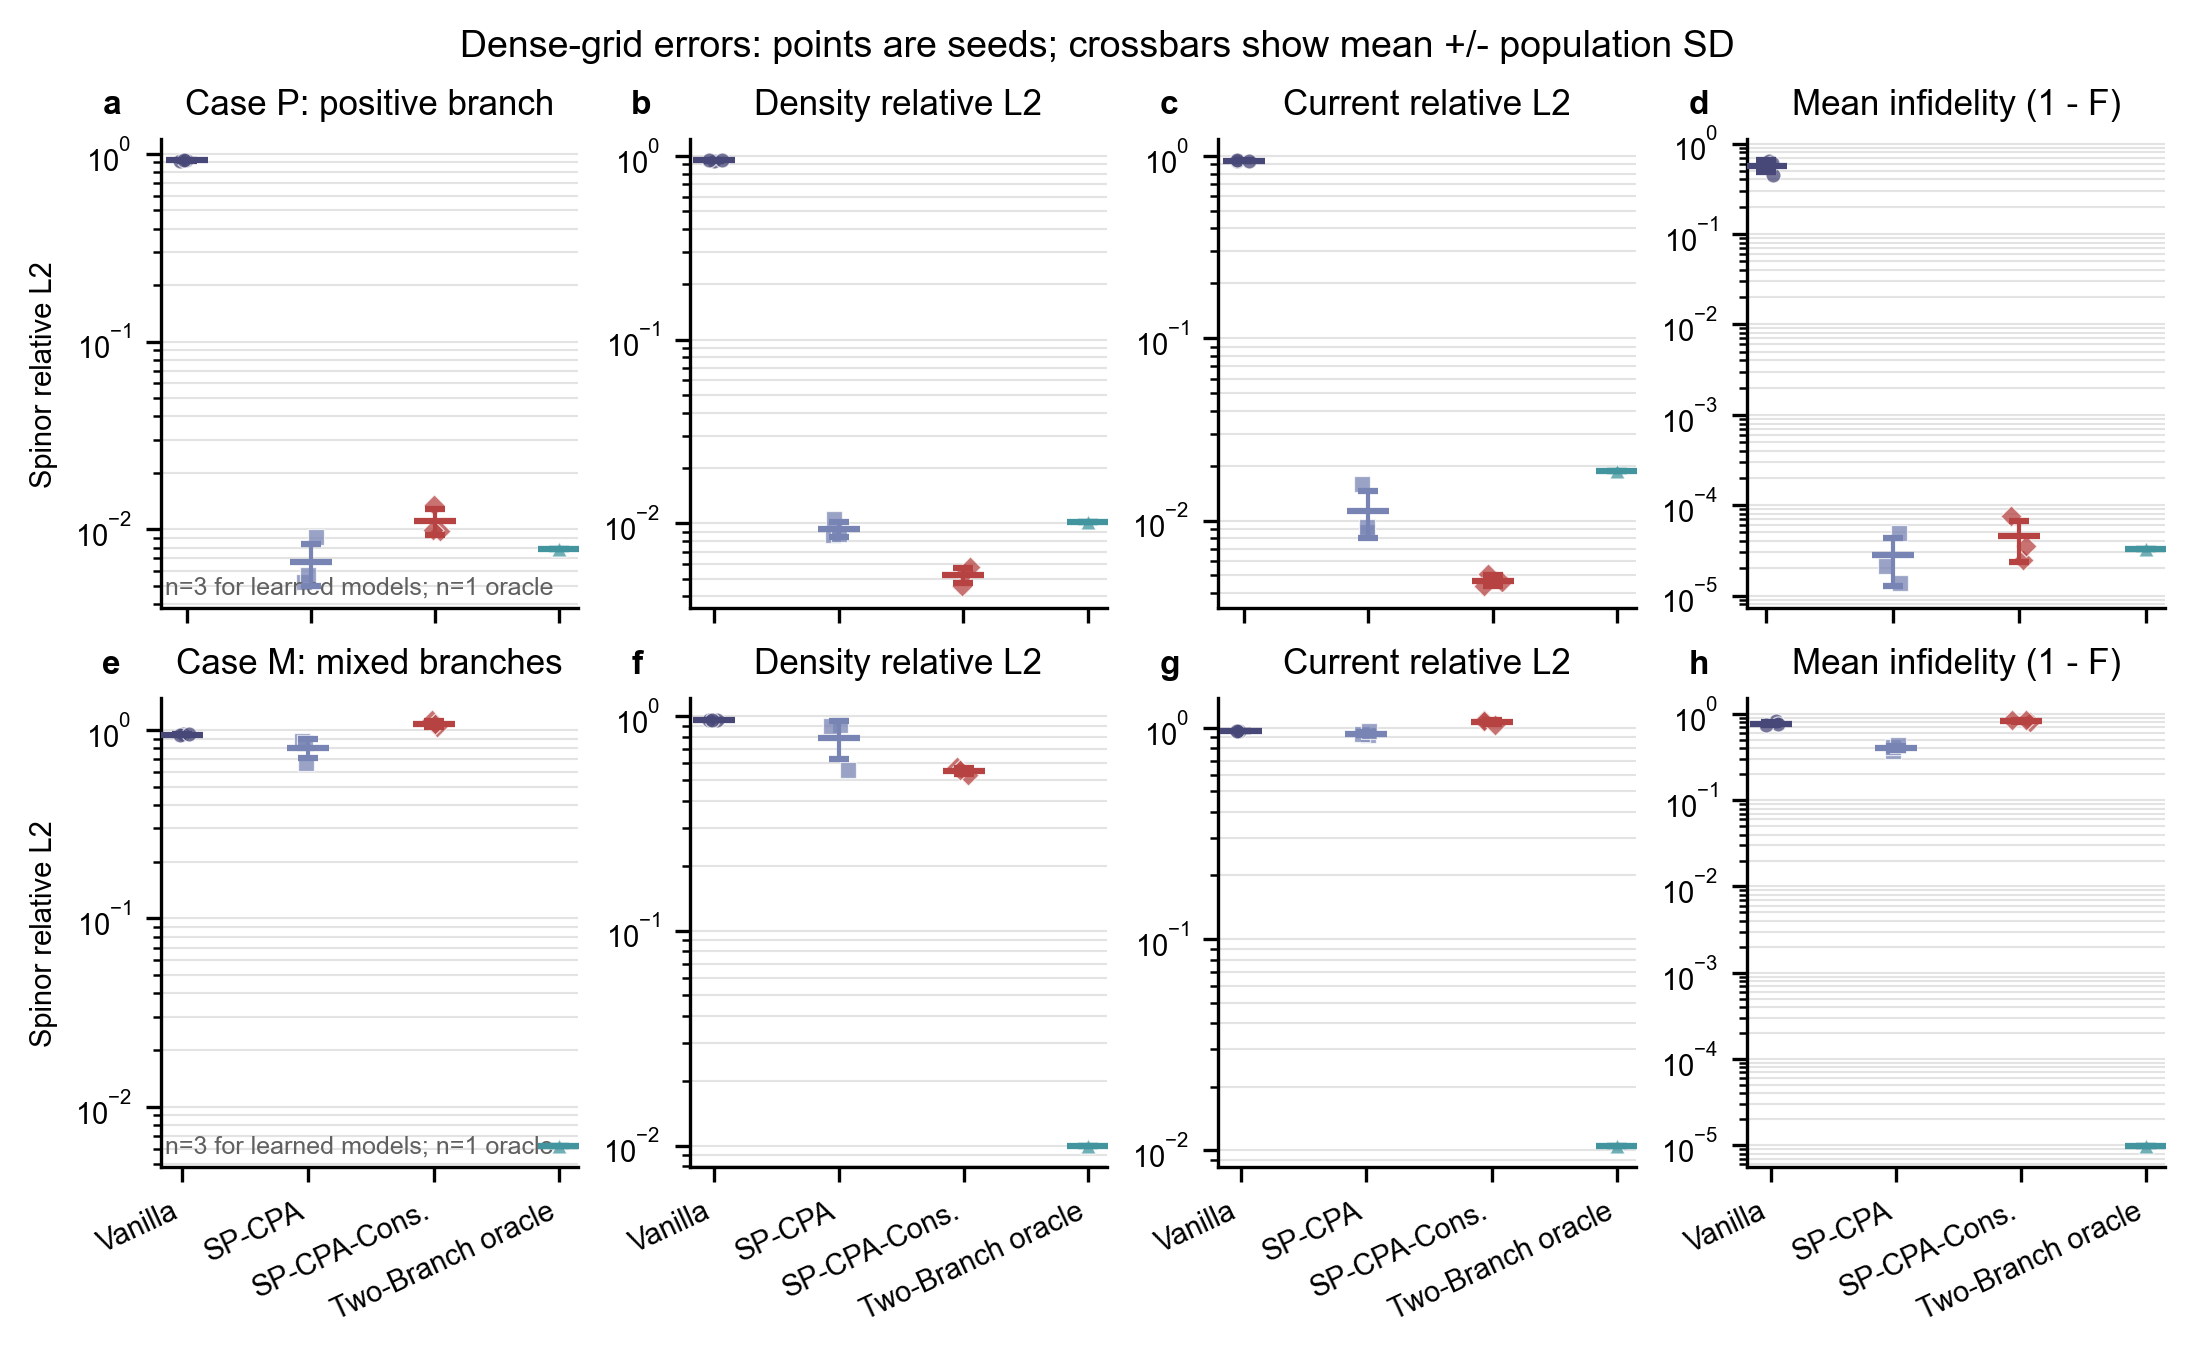
\includegraphics[width=\linewidth]{results/figures/01_main_metric_comparison.png}
\end{column}
\begin{column}{0.30\textwidth}
\scriptsize
\renewcommand{\arraystretch}{1.12}
\begin{tabular}{@{}lrr@{}}
\toprule
Model & P error & M error \\
\midrule
Vanilla & 0.9228 & 0.9452 \\
SP-CPA & \textbf{0.0067} & 0.7991 \\
SP-CPA-Con. & 0.0111 & 1.0785 \\
Two-frequency & 0.0079 & \textbf{0.0062} \\
\bottomrule
\end{tabular}

\vspace{0.7em}
\begin{block}{Interpretation}
SP-CPA reduces the Case-P spinor error by 99.3\%, but only by 15.5\% in Case M.
Conservation penalties do not restore the missing relative phase.
\end{block}
\end{column}
\end{columns}

\vspace{0.2em}
\centering
\small The transfer failure is representation-dependent, rather than a generic
failure of physics-informed training.
\end{frame}

\section{Method}

\begin{frame}{Stage III: Learnable Two-Phase Branch-Aligned PINN}
The spectral projectors of the free Dirac Hamiltonian are
\begin{equation*}
P_\pm(k)=\frac{1}{2}\left(I_2\pm\frac{H(k)}{E(k)}\right),
\qquad P_+P_-=0,
\qquad P_++P_-=I_2.
\end{equation*}
LTPB represents each energy eigenspace with its own amplitude and phase:
\begin{equation*}
\widehat\psi(k,t)=
a_+(k,t)u_+(k)e^{iS_+(k,t)}+
a_-(k,t)u_-(k)e^{iS_-(k,t)}.
\end{equation*}

\begin{columns}[T,onlytextwidth]
\begin{column}{0.49\textwidth}
\begin{block}{Training information}
The exact frequency \(E(k)\) is not supplied as phase supervision. The phases
are identified from the Dirac residual, initial data, and normalization or
gauge conditions.
\end{block}
\end{column}
\begin{column}{0.47\textwidth}
\begin{block}{Physical mechanism}
The current contains cross terms governed by
\(S_-(k,t)-S_+(k,t)\). Independent phases can therefore represent the
interference oscillation explicitly.
\end{block}
\end{column}
\end{columns}
\end{frame}

\begin{frame}{LTPB Pilot: Accuracy and Identified Phases}
\begin{columns}[T,onlytextwidth]
\begin{column}{0.50\textwidth}
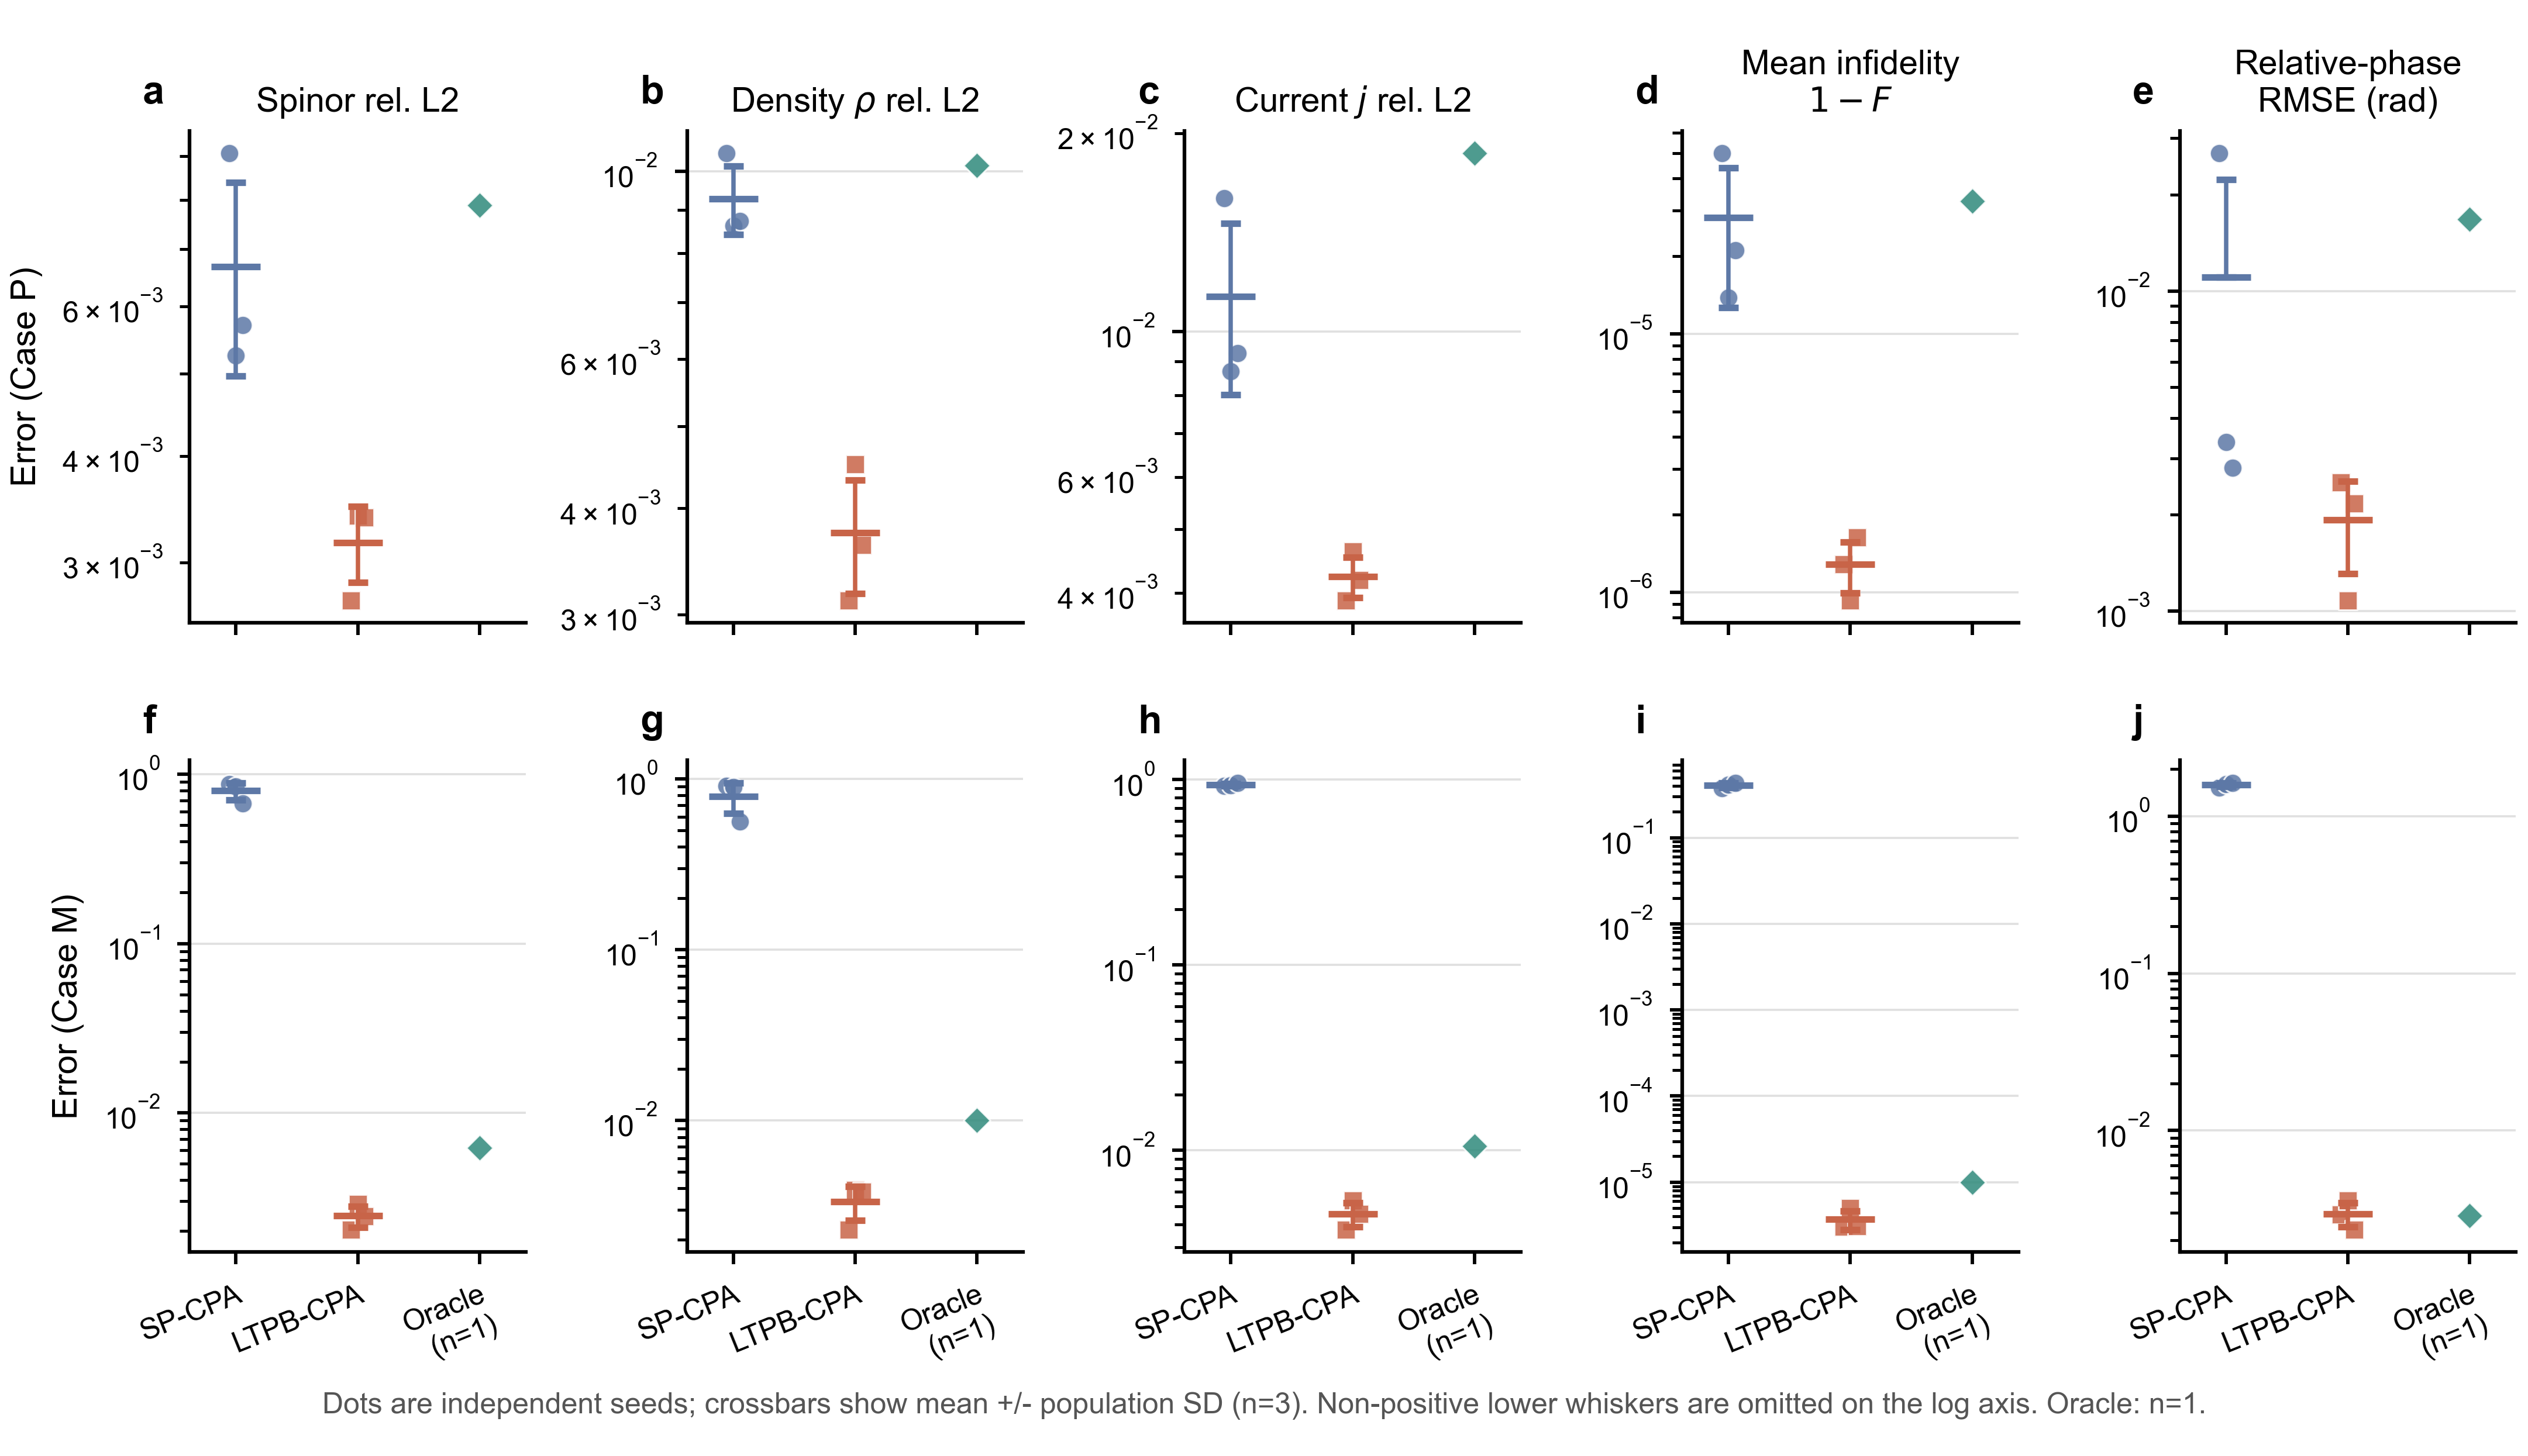
\includegraphics[width=\linewidth]{results/figures/learned_two_phase_pilot/01_main_metric_comparison.png}
\centering\scriptsize Error comparison for pure- and mixed-energy states
\end{column}
\begin{column}{0.48\textwidth}
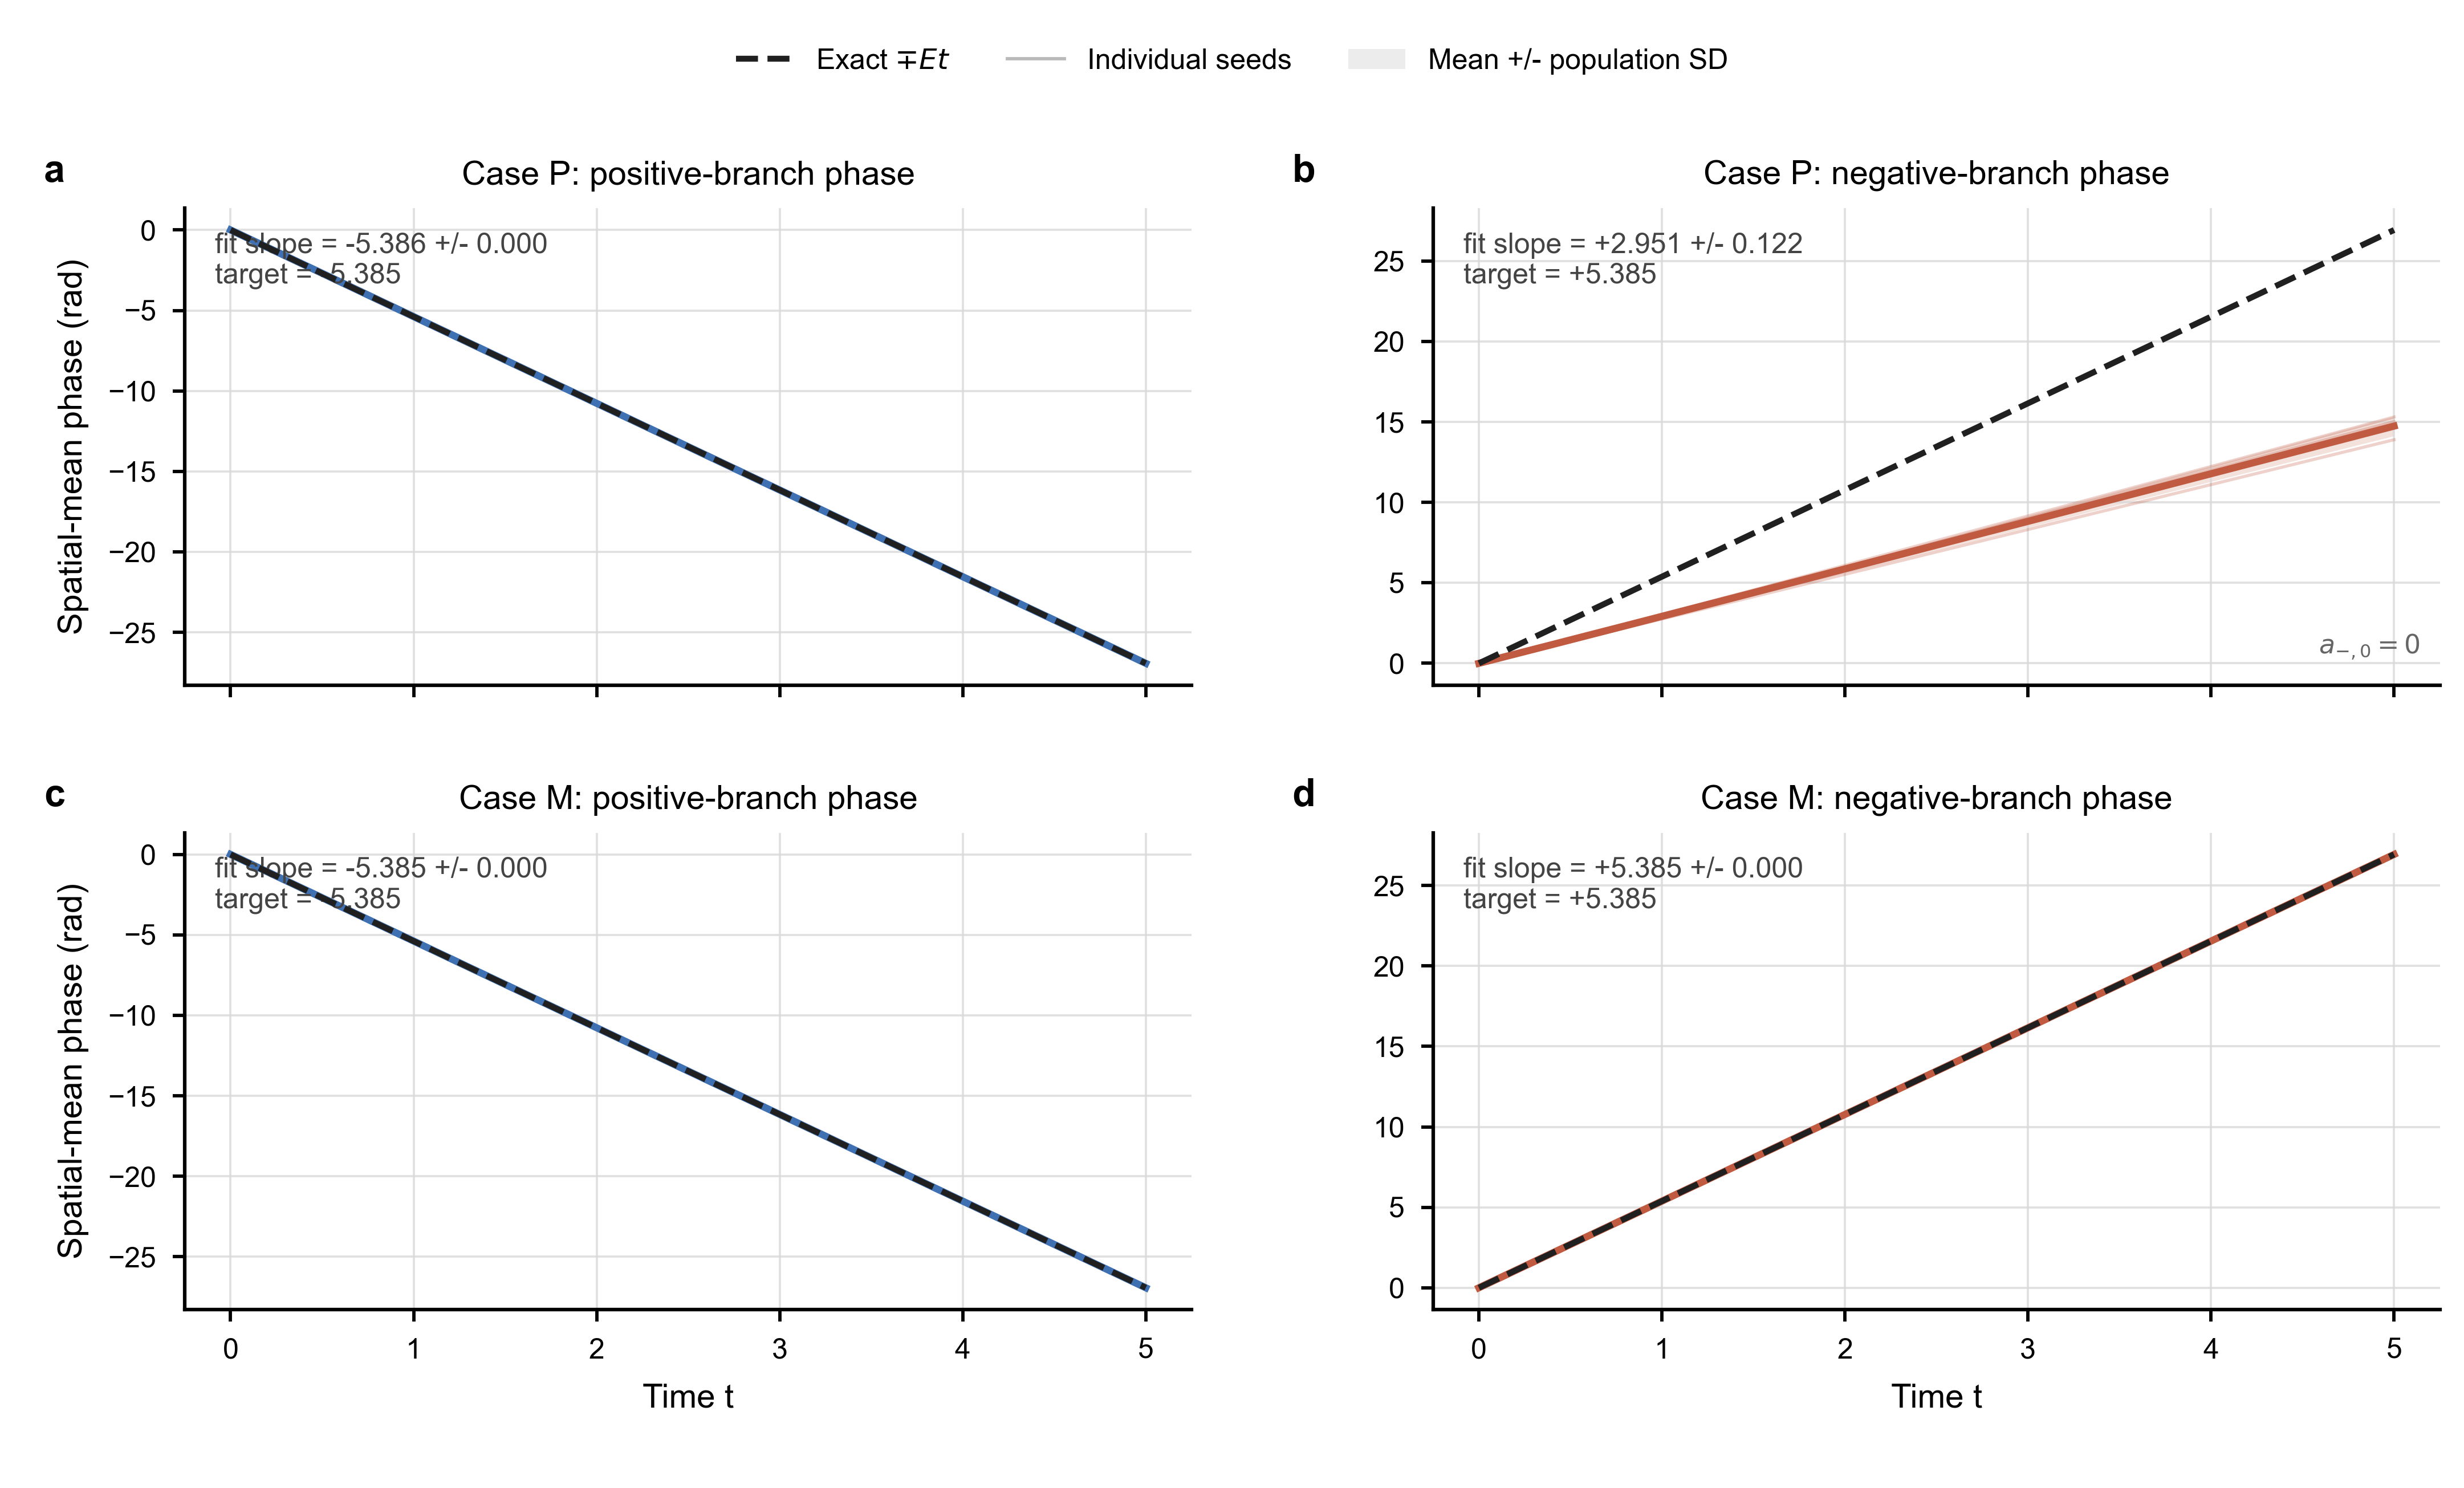
\includegraphics[width=\linewidth]{results/figures/learned_two_phase_pilot/02_learned_branch_phases.png}
\centering\scriptsize Learned slopes approach \(-E\) and \(+E\)
\end{column}
\end{columns}

\vspace{0.5em}
\scriptsize
\centering
\renewcommand{\arraystretch}{1.12}
\begin{tabular}{@{}lrrrr@{}}
\toprule
Method & Spinor error & Current error & Phase RMSE & Fidelity \\
\midrule
SP-CPA & 0.7991 & 0.9392 & 1.5864 & 0.5935 \\
LTPB & \textbf{0.0025} & \textbf{0.0046} & \textbf{0.0030} & \textbf{0.999996} \\
\bottomrule
\end{tabular}

\vspace{0.35em}
\small Identified phase slopes: \(-5.3855\) and \(+5.3854\), versus the exact
values \(\mp5.3851648\).
\end{frame}

\begin{frame}{Stage IV: Which Structure Is Essential?}
\begin{columns}[T,onlytextwidth]
\begin{column}{0.43\textwidth}
\scriptsize
\renewcommand{\arraystretch}{1.12}
\begin{tabular}{@{}lrr@{}}
\toprule
Model & Spinor & Current \\
\midrule
LTPB & \textbf{0.0025} & \textbf{0.0045} \\
BranchComplex & 0.9014 & 0.9342 \\
ComponentPolar & 0.8907 & 0.9309 \\
Rotated \(15^\circ\) & 0.8996 & 0.9426 \\
Rotated \(30^\circ\) & 0.9306 & 0.9590 \\
\bottomrule
\end{tabular}

\vspace{0.6em}
All models contain approximately 12,996 trainable parameters and use paired
initializations and collocation sequences.
\end{column}
\begin{column}{0.55\textwidth}
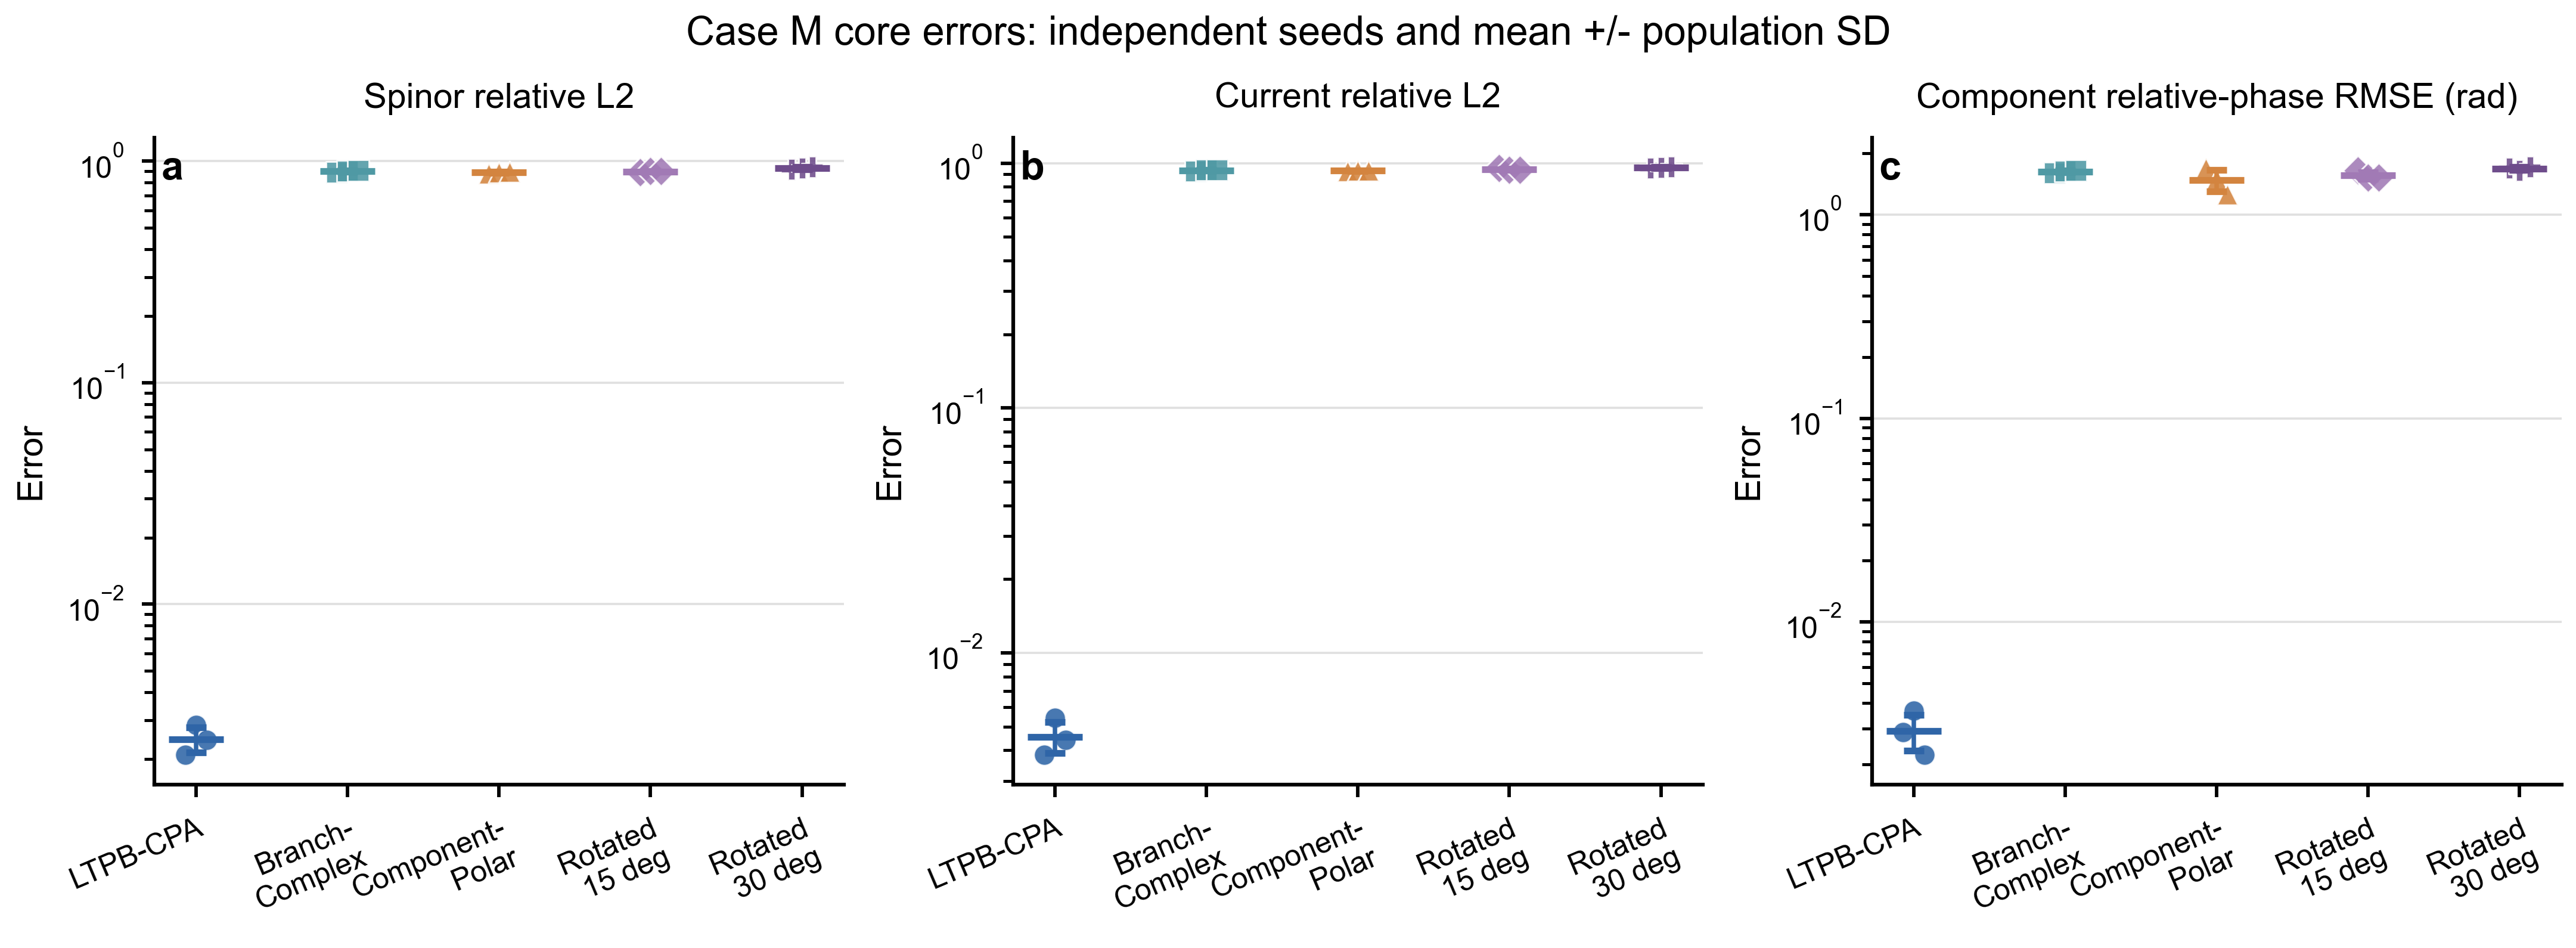
\includegraphics[width=\linewidth]{results/figures/ltpb_mechanism_ablation/01_core_error_comparison.png}
\end{column}
\end{columns}

\begin{block}{Supported mechanistic conclusion}
Low error requires the joint use of energy-eigenspace alignment and independent
phase functions. The preregistered monotone \(1.25\times\) rotation-degradation
criterion was not met because the error had already reached a high plateau at
\(15^\circ\).
\end{block}
\end{frame}

\section{Generalization}

\begin{frame}{Stage V: Two Wavenumbers and Four Energy Components}
For \(k_1=2\) and \(k_2=5\), the reference state is
\begin{equation*}
\psi(x,t)=\frac{1}{2\sqrt L}\sum_{l=1}^{2}
\left[u_+(k_l)e^{ik_lx-iE_lt}+u_-(k_l)e^{ik_lx+iE_lt}\right].
\end{equation*}
Multi-LTPB assigns one learnable phase to each \((k_l,\pm)\) component without
using the exact \(E_l\).

\begin{columns}[T,onlytextwidth]
\begin{column}{0.48\textwidth}
\begin{block}{Controlled comparison}
Five trainable models use nearly identical parameter counts, 5000 optimization
steps, and five paired random seeds.
\end{block}
\end{column}
\begin{column}{0.48\textwidth}
\scriptsize
\renewcommand{\arraystretch}{1.12}
\begin{tabular}{@{}lrr@{}}
\toprule
Metric & Multi-LTPB & Best baseline \\
\midrule
Spinor error & \textbf{0.006594} & 0.939819 \\
Current error & \textbf{0.010976} & 0.957364 \\
Fidelity & \textbf{0.999965} & 0.3172 \\
Paired seeds & \textbf{5/5 pass} & -- \\
\bottomrule
\end{tabular}
\end{column}
\end{columns}
\end{frame}

\begin{frame}{Discrete Multimode Results}
\begin{columns}[T,onlytextwidth]
\begin{column}{0.52\textwidth}
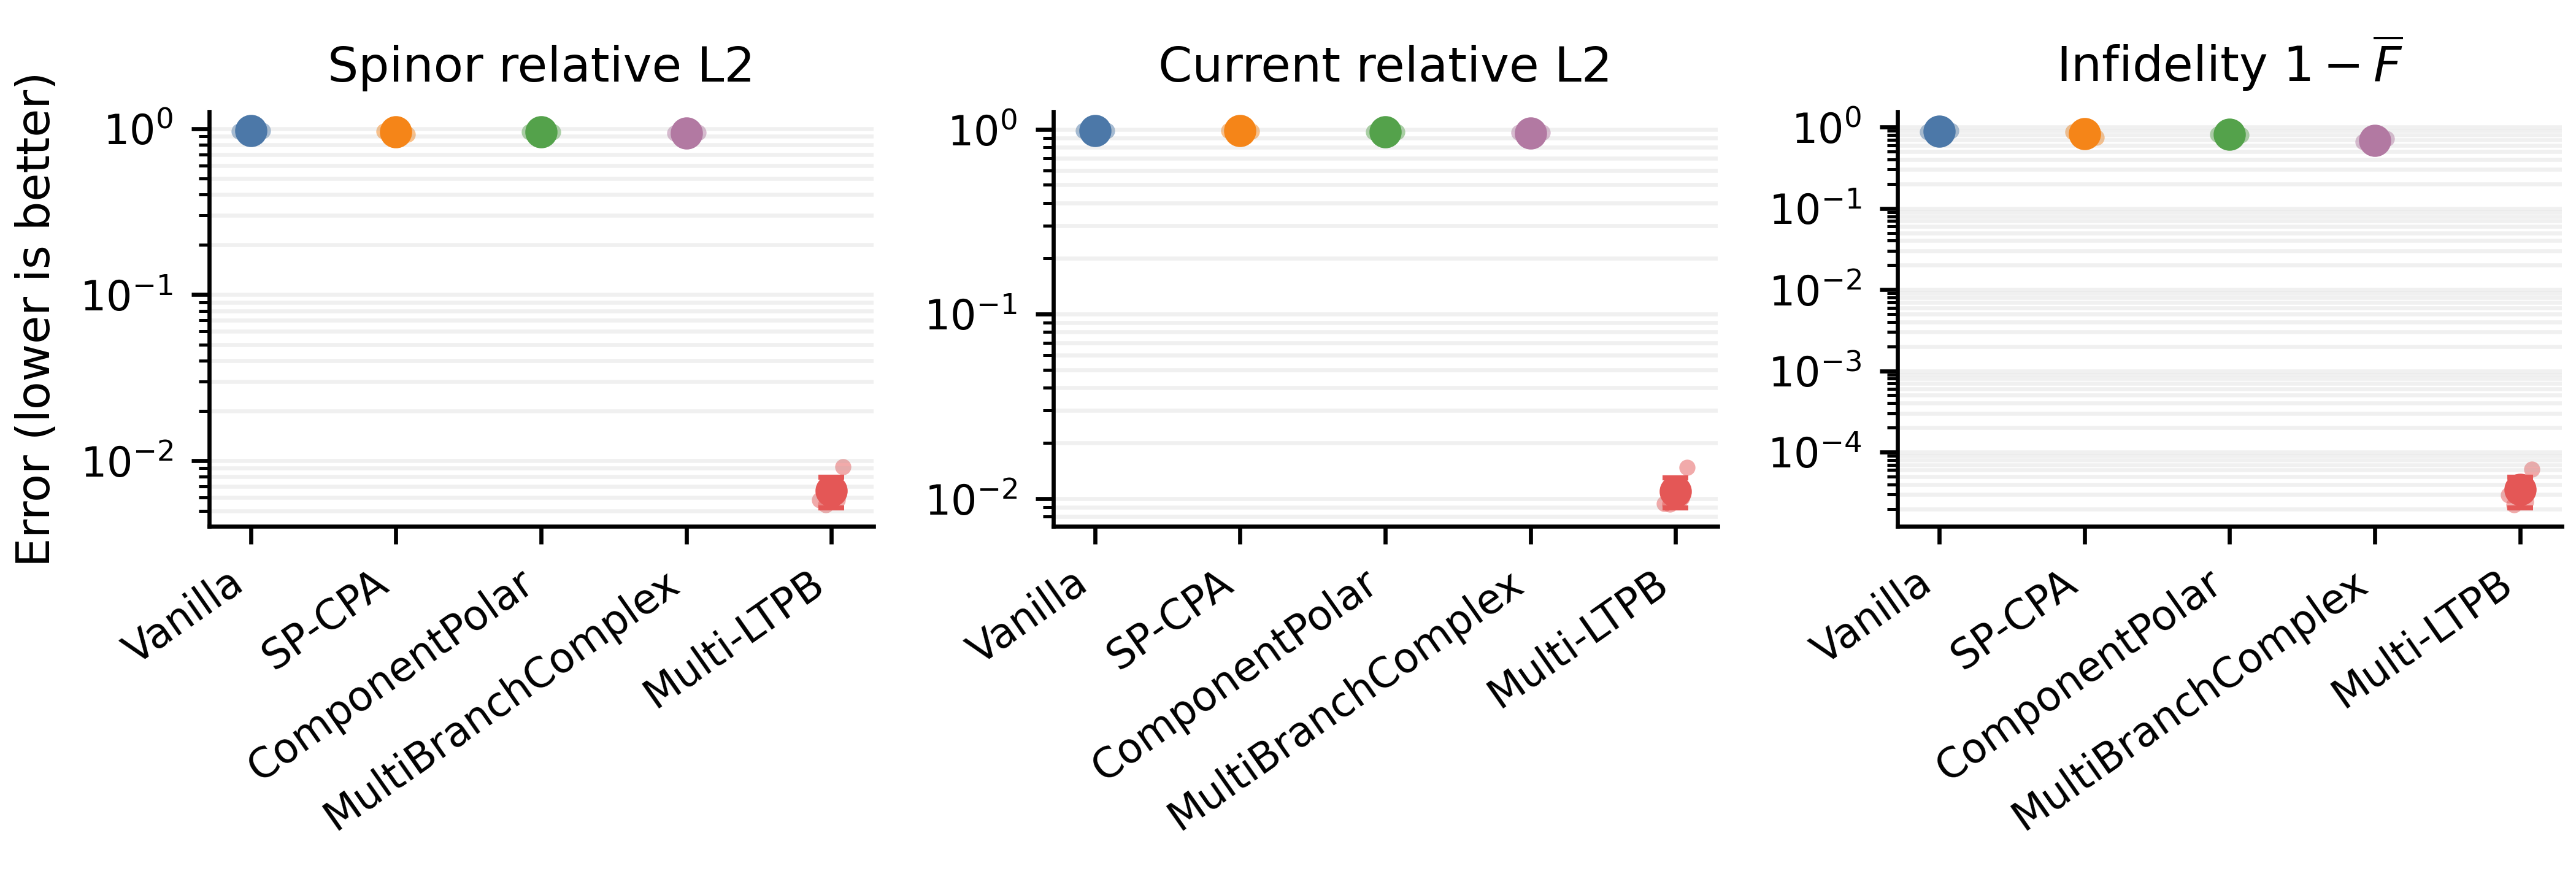
\includegraphics[width=\linewidth]{results/figures/multimode_ltpb/primary_error_comparison.png}
\centering\scriptsize Primary error comparison
\end{column}
\begin{column}{0.46\textwidth}
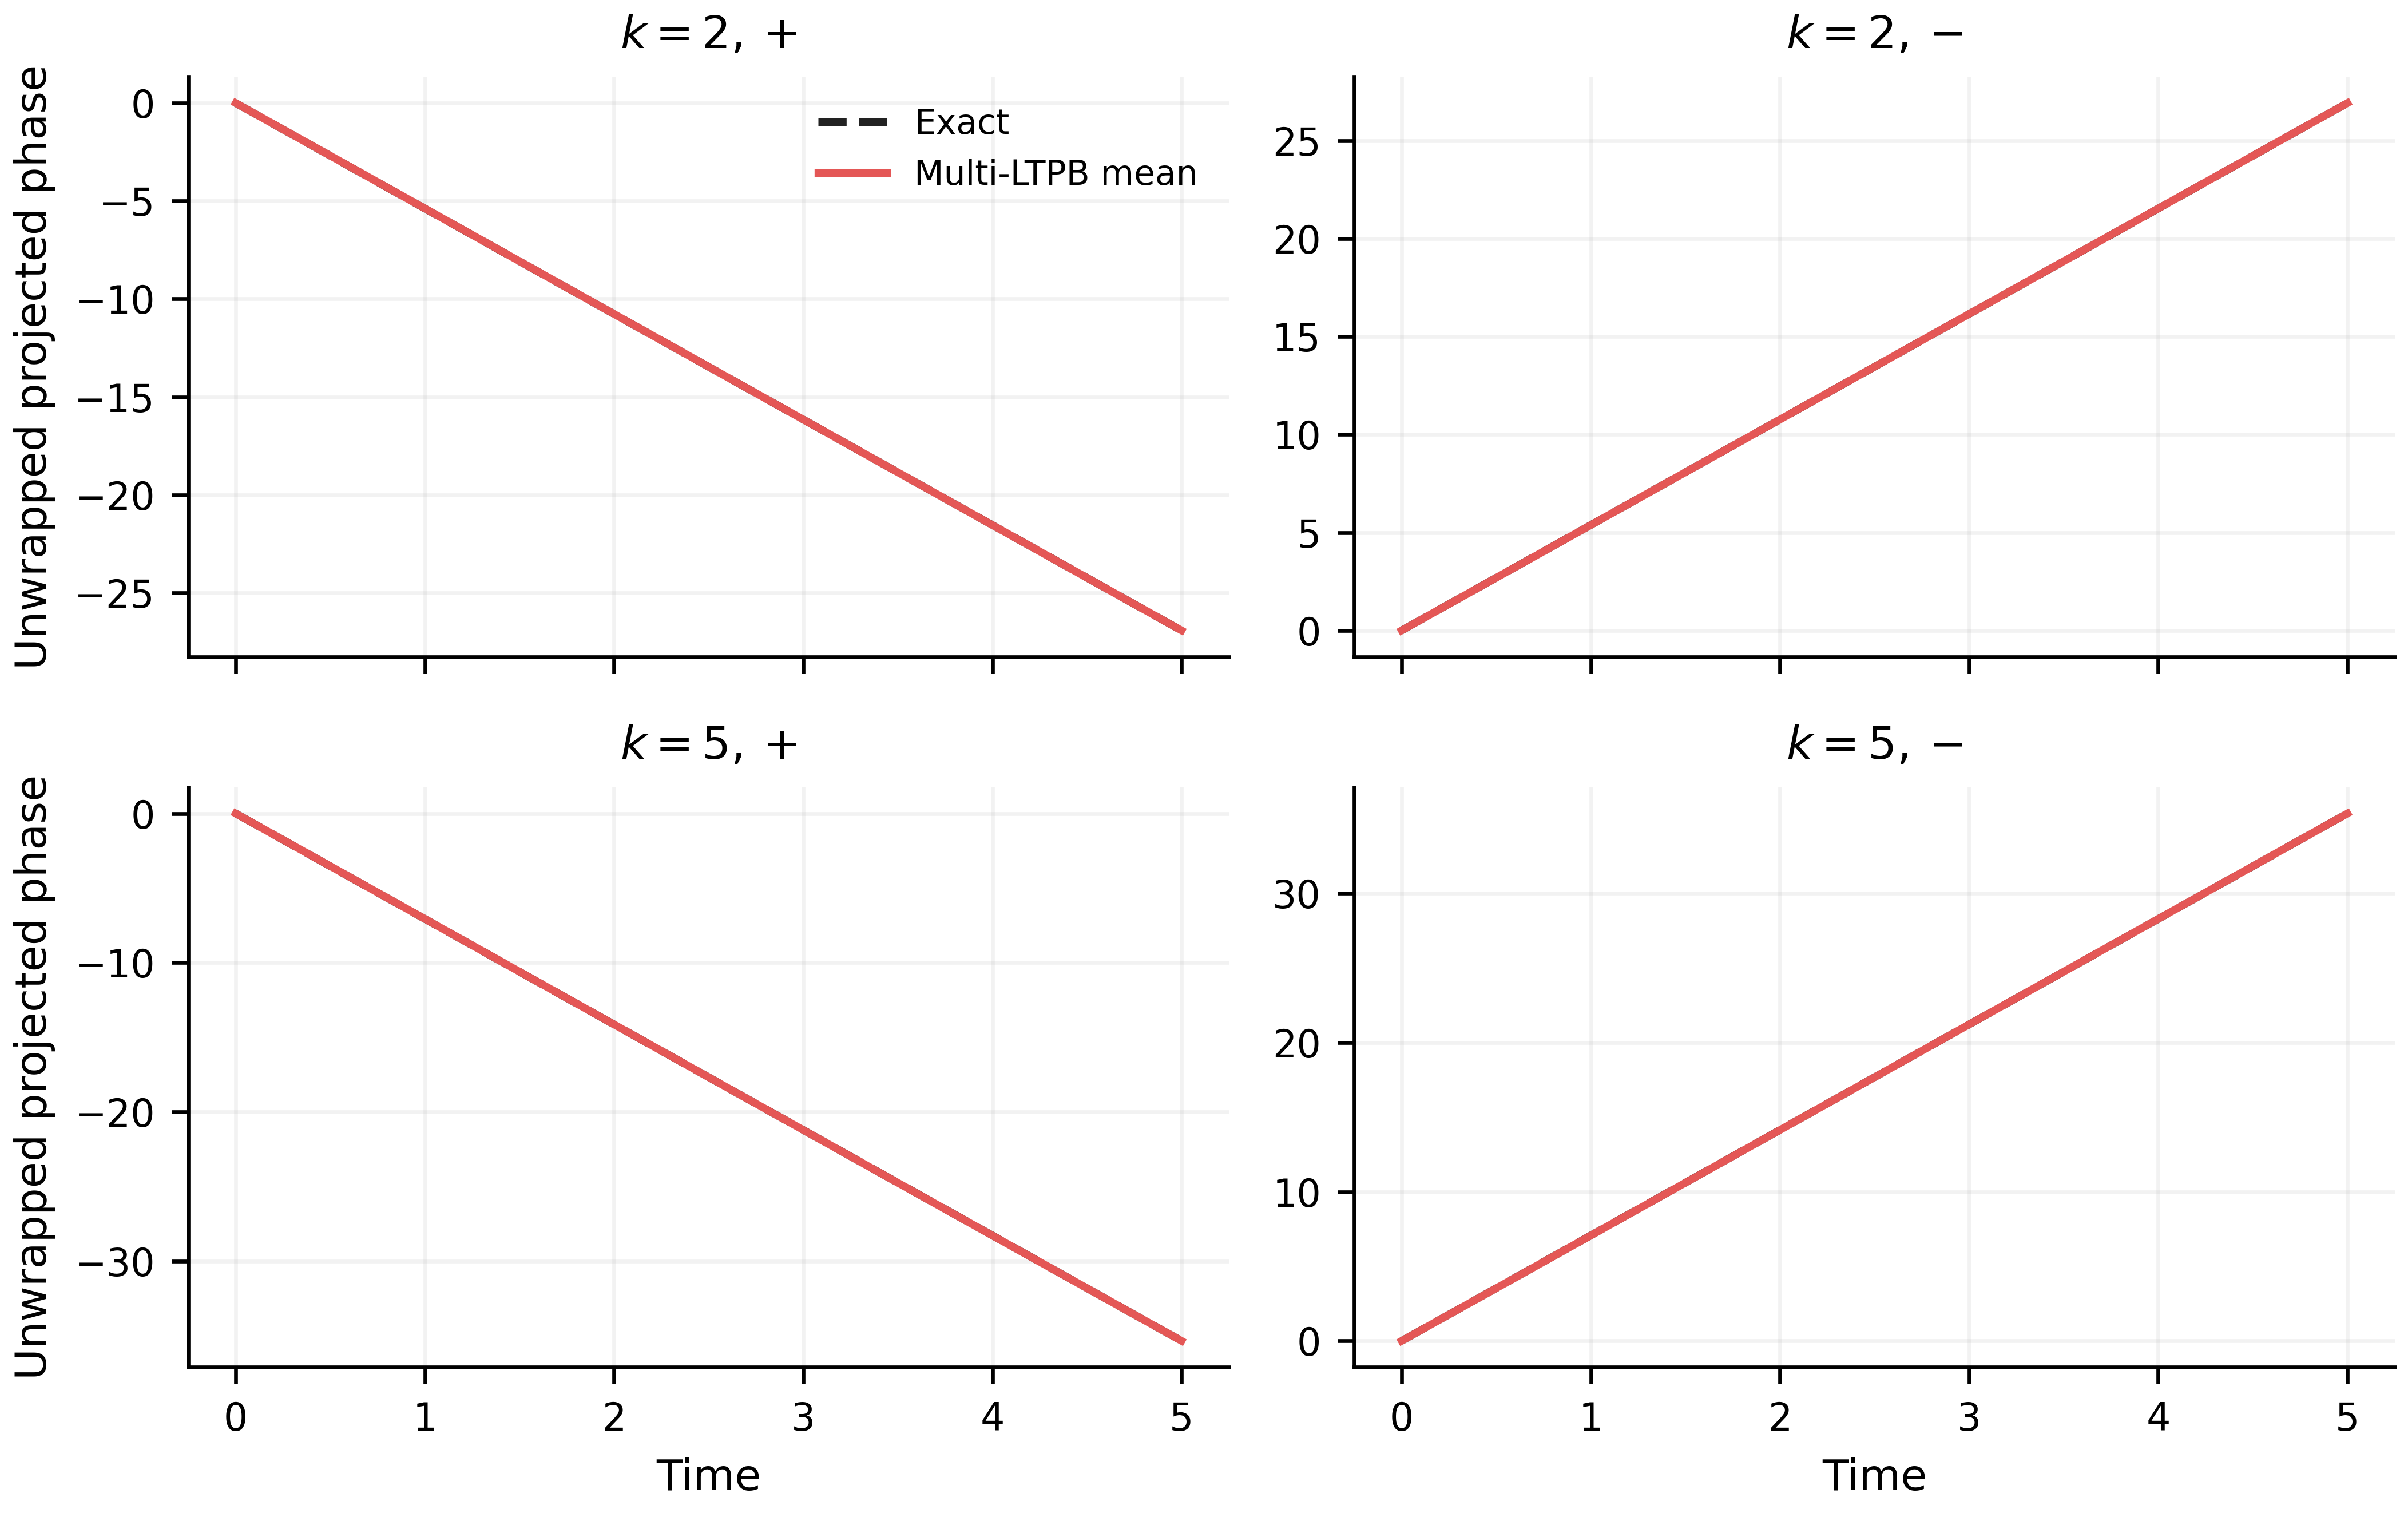
\includegraphics[width=\linewidth]{results/figures/multimode_ltpb/learned_four_phases.png}
\centering\scriptsize Four learned phase functions
\end{column}
\end{columns}

\vspace{0.6em}
\begin{block}{Stage-V conclusion}
The phase-separated, eigenspace-aligned representation remains accurate when
both spectral multiplicity and the number of energy components increase. The
spinor and current errors improve over the best trainable baseline by factors
of 142.52 and 87.22, respectively.
\end{block}
\end{frame}

\begin{frame}{Stage VI: Shared-Spectral Wave-Packet Formulation}
A Gaussian momentum distribution is sampled by 33 wavenumbers
\(k_n=n/8\in[0,4]\), with center \(k_0=2\), width \(\sigma_k=0.5\), and equal
positive- and negative-energy weights.

\begin{equation*}
\widehat{\widetilde\psi}(k,t)=
a_+(k,t)u_+(k)e^{iS_+(k,t)}+
a_-(k,t)u_-(k)e^{iS_-(k,t)}.
\end{equation*}
One network takes \((k,t)\) as input and shares its parameters over all modes.
The spectral residual is
\begin{equation*}
R_k=i\partial_t\widehat{\widetilde\psi}
-\left(k\sigma_x+m\sigma_z\right)\widehat{\widetilde\psi}.
\end{equation*}

\begin{block}{Scalability principle}
The parameter count remains 12,932 and does not grow linearly with the number
of represented Fourier modes. The exact dispersion \(E(k)\) is not supplied as
phase supervision.
\end{block}
\end{frame}

\begin{frame}{Continuous Wave Packet: Primary Results}
\begin{columns}[T,onlytextwidth]
\begin{column}{0.62\textwidth}
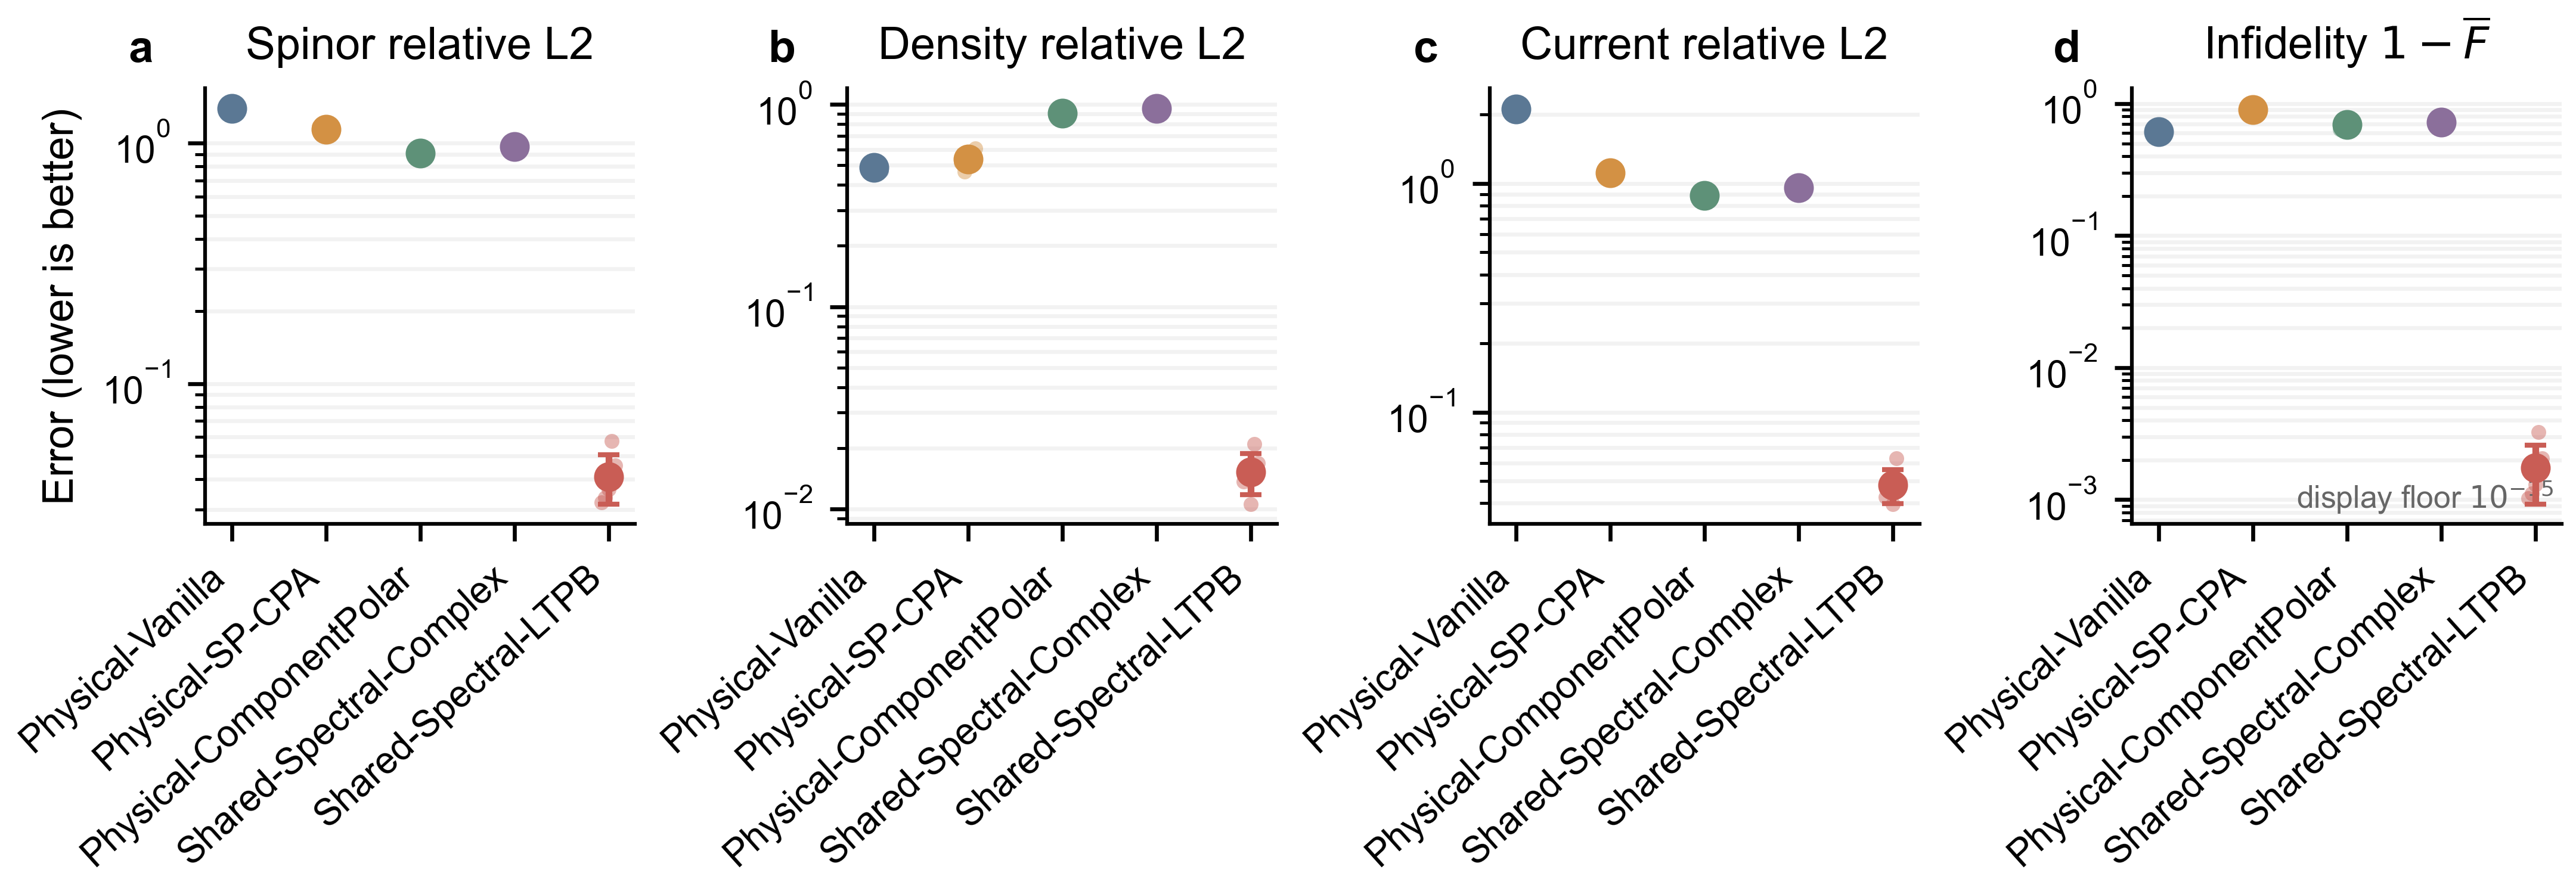
\includegraphics[width=\linewidth]{results/figures/wavepacket_shared_spectral_ltpb/primary_error_comparison.png}
\end{column}
\begin{column}{0.36\textwidth}
\scriptsize
\renewcommand{\arraystretch}{1.13}
\begin{tabular}{@{}lr@{}}
\toprule
Metric & Shared-Spectral \\
\midrule
Spinor error & \textbf{0.041038} \\
Density error & \textbf{0.015262} \\
Current error & \textbf{0.048057} \\
Fidelity & \textbf{0.998249} \\
Paired seeds & \textbf{5/5 pass} \\
\bottomrule
\end{tabular}

\vspace{0.8em}
The spinor and current errors are lower than those of the best trainable
baseline by factors of 22.16 and 18.40.
\end{column}
\end{columns}

\vspace{0.25em}
\centering\small Accuracy remains high as the model moves from a discrete
spectrum to a prescribed continuous spectral interval.
\end{frame}

\begin{frame}{Dispersion Generalization and Packet Transport}
\begin{columns}[T,onlytextwidth]
\begin{column}{0.49\textwidth}
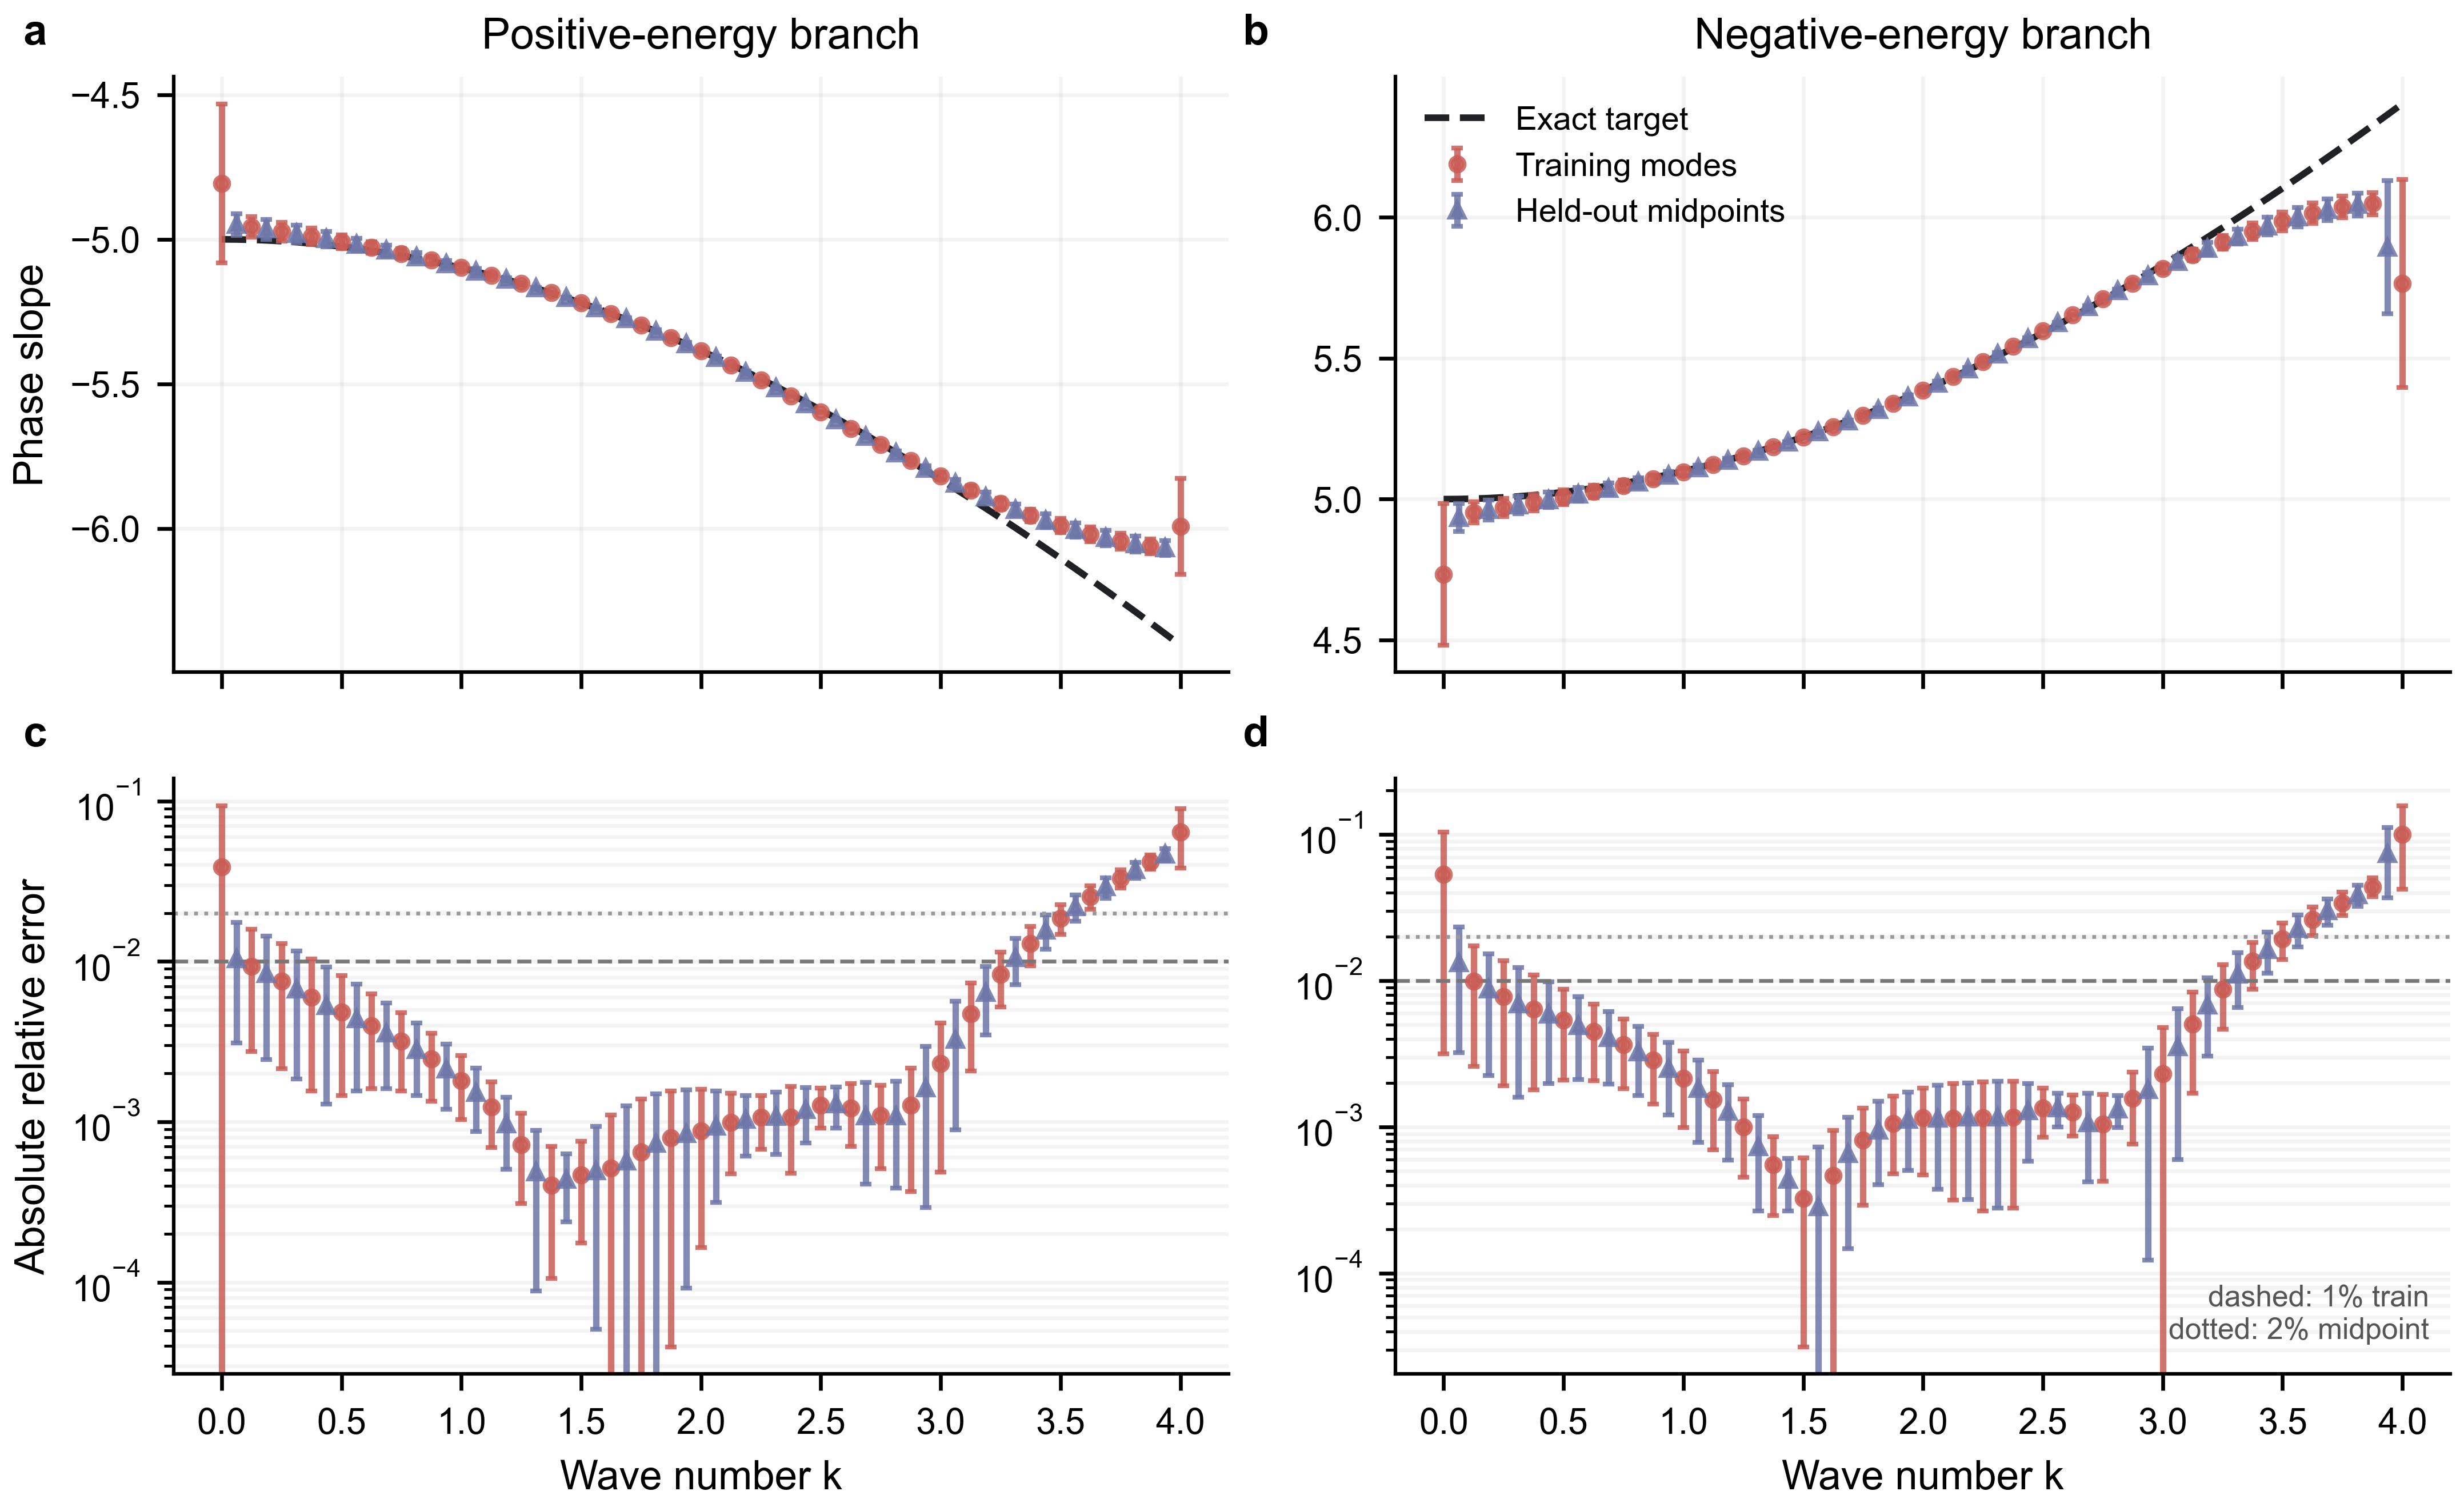
\includegraphics[width=\linewidth]{results/figures/wavepacket_shared_spectral_ltpb/phase_slope_train_midpoint.png}
\centering\scriptsize Phase slopes at training and unseen midpoint wavenumbers
\end{column}
\begin{column}{0.49\textwidth}
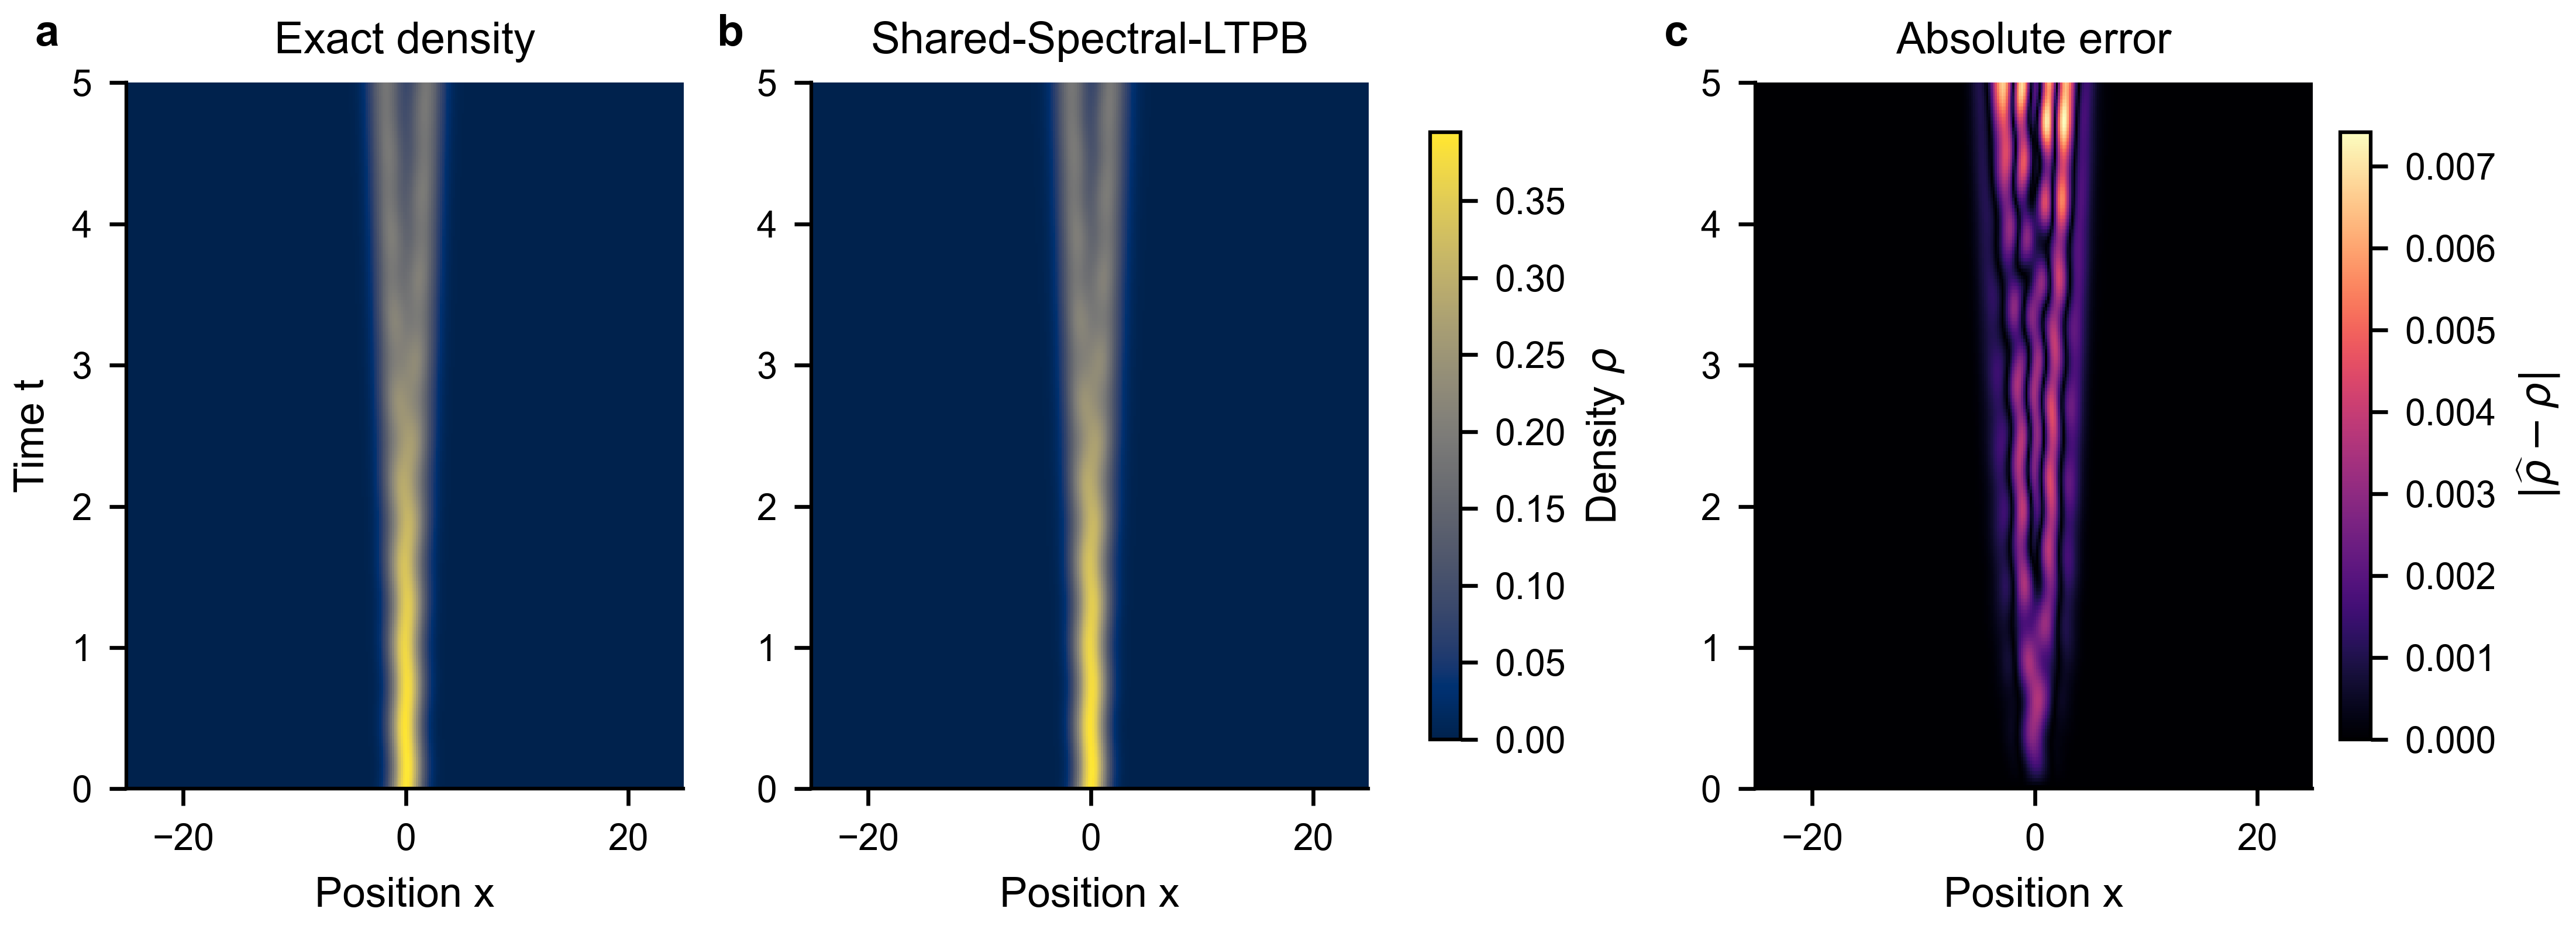
\includegraphics[width=\linewidth]{results/figures/wavepacket_shared_spectral_ltpb/wavepacket_density_spacetime.png}
\centering\scriptsize Reference and learned density evolution
\end{column}
\end{columns}

\vspace{0.6em}
\begin{itemize}
  \item Mean phase-slope error: \(0.115\%\) at training points and unseen midpoints.
  \item Mean group velocities: \(+0.3665\) and \(-0.3659\) for the two packets.
  \item Residual RMSE at unseen midpoint wavenumbers: \(0.0017\)--\(0.0033\).
\end{itemize}
\end{frame}

\begin{frame}{Evidence Across Increasing Spectral Complexity}
\centering
\small
\renewcommand{\arraystretch}{1.18}
\begin{tabularx}{\textwidth}{@{}Ylrrr@{}}
\toprule
Problem & Method & Spinor error & Current error & Fidelity \\
\midrule
Single-wavenumber mixed-energy state & LTPB & 0.0025 & 0.0046 & 0.999996 \\
Two wavenumbers, four components & Multi-LTPB & 0.0066 & 0.0110 & 0.999965 \\
33-mode Gaussian packet & Shared-Spectral-LTPB & 0.0410 & 0.0481 & 0.998249 \\
\bottomrule
\end{tabularx}

\vspace{1.0em}
\begin{block}{Evidence supported by the completed experiments}
For the one-dimensional free Dirac equation, a prescribed Fourier expansion,
and fixed training budgets, independent learnable phases aligned with the two
energy eigenspaces substantially reduce spinor, current, and relative-phase
errors for mixed-energy states.
\end{block}

\begin{alertblock}{Current boundary}
The error rises as spectral width increases. Robustness under dynamically
coupled momentum channels has not yet been established.
\end{alertblock}
\end{frame}

\section{Positioning}

\begin{frame}{Relation to Existing Methods}
\scriptsize
\renewcommand{\arraystretch}{1.16}
\begin{tabularx}{\textwidth}{@{}lYYY@{}}
\toprule
Method class & Established strength & Limitation addressed here & Present position of LTPB \\
\midrule
CPA-PINN for semiclassical Schr\"odinger/NLS equations &
Common phase-amplitude coordinates with conservation constraints &
A single phase does not isolate both Dirac energy signs &
Retains rapid-phase extraction but aligns separate phases with spectral projectors \\
General Dirac PINN &
Direct spinor representation with limited prior spectral assumptions &
Strong temporal oscillation remains inside network outputs &
Introduces a stronger coordinate system when the free spectral structure is known \\
Fourier and split-operator solvers &
High-accuracy forward propagation with mature error analysis &
Do not primarily target equation-data fusion or continuous neural surrogates &
No demonstrated single-query cost advantage; prospective value is inference and sparse-data assimilation \\
\bottomrule
\end{tabularx}

\vspace{0.7em}
\begin{block}{Prospective algorithmic advantage}
The completed experiments indicate improved optimization conditioning and
long-time phase accuracy for spectrally resolvable mixed-energy states. Claims
of broader superiority require external-potential, data-constrained, and cost
benchmarks.
\end{block}
\end{frame}

\section{Next Stage}

\begin{frame}{Stage VII: Weak Smooth Periodic Potential}
The next experiment introduces
\begin{equation*}
V(x)=V_0\cos(qx)I_2,
\end{equation*}
which couples neighboring momentum channels:
\begin{equation*}
i\partial_t\widetilde\psi_k=
H(k)\widetilde\psi_k+\frac{V_0}{2}
\left(\widetilde\psi_{k-q}+\widetilde\psi_{k+q}\right).
\end{equation*}

\begin{columns}[T,onlytextwidth]
\begin{column}{0.48\textwidth}
\textbf{Primary observables}
\begin{itemize}
  \item Modal population exchange.
  \item Density and current density.
  \item Coherence between energy components.
  \item Long-time phase and norm drift.
\end{itemize}
\end{column}
\begin{column}{0.48\textwidth}
\textbf{New algorithmic difficulty}
\begin{itemize}
  \item Momentum channels are dynamically generated.
  \item Polar phase becomes ill-conditioned near zero amplitude.
  \item Candidate remedy: amplitude-aware phase regularization or hybrid
  complex/polar coordinates.
\end{itemize}
\end{column}
\end{columns}
\end{frame}

\begin{frame}{Unified Benchmark Required for Submission}
\begin{columns}[T,onlytextwidth]
\begin{column}{0.32\textwidth}
\begin{block}{Baselines}
\begin{itemize}
  \item Vanilla and adaptive PINNs.
  \item Loss-balancing PINNs.
  \item SP-CPA and ablated LTPB variants.
  \item Fourier pseudospectral solver.
  \item Split-operator solver.
\end{itemize}
\end{block}
\end{column}
\begin{column}{0.32\textwidth}
\begin{block}{Evaluation}
\begin{itemize}
  \item Spinor, density, and current errors.
  \item Fidelity and relative phase.
  \item Long-time norm drift.
  \item Seed-level variability.
  \item Wall time, memory, and parameter count.
\end{itemize}
\end{block}
\end{column}
\begin{column}{0.32\textwidth}
\begin{block}{Data-Constrained Study}
\begin{itemize}
  \item Sparse noisy \(\rho\) or \(j\) observations.
  \item State reconstruction.
  \item Inference of \(m\), \(V_0\), and \(q\).
  \item Noise-level and sensor-density sweeps.
  \item Identifiability diagnostics.
\end{itemize}
\end{block}
\end{column}
\end{columns}

\begin{alertblock}{Minimum evidence for a complete paper}
At least one coupled external-potential problem, one sparse noisy-data inverse
problem, classical-solver references, mechanism ablations, and a complete cost
analysis.
\end{alertblock}
\end{frame}

\section{Conclusion}

\begin{frame}{Conclusions}
\begin{enumerate}
  \item A single common phase is effective for a pure energy component but loses
  most of its fixed-budget benefit for mixed positive/negative-energy states.
  \item LTPB resolves the spinor in the two energy eigenspaces and assigns an
  independent learnable phase to each component.
  \item Parameter-matched ablations identify eigenspace alignment and phase
  separation as jointly necessary on the present benchmark.
  \item The construction has progressed from one mode to four components and a
  33-mode Gaussian packet while preserving high fidelity.
  \item The decisive next test is a periodic external potential, where momentum
  transfer and near-zero modal amplitudes challenge the current coordinates.
\end{enumerate}

\begin{block}{Present assessment}
The completed results establish a coherent free-Dirac proof of concept. A
journal-level claim requires coupled dynamics, data-constrained inference, and
comparison with mature numerical solvers.
\end{block}
\end{frame}

\begin{frame}{Selected References}
\footnotesize
\begin{thebibliography}{9}
\bibitem{Kumar2026}
S. Kumar, H. K. Dwivedi, and Rajeev,
``Structure-preserving conservative phase-amplitude PINNs for semiclassical
Schr\"odinger-type equations,''
\emph{Journal of Computational and Applied Mathematics}, vol. 485, 117607,
2026. DOI: 10.1016/j.cam.2026.117607.

\bibitem{Lorin2022}
E. Lorin and X. Yang,
``Time-dependent Dirac equation with physics-informed neural networks:
Computation and properties,''
\emph{Computer Physics Communications}, vol. 280, 108474, 2022.
DOI: 10.1016/j.cpc.2022.108474.

\bibitem{Bao2016}
W. Bao, Y. Cai, X. Jia, and Q. Tang,
``A uniformly accurate multiscale time integrator pseudospectral method for the
Dirac equation in the nonrelativistic limit regime,''
\emph{SIAM Journal on Numerical Analysis}, vol. 54, no. 3, pp. 1785--1812,
2016. DOI: 10.1137/15M1032375.
\end{thebibliography}

\vfill
\centering
All numerical figures are reproduced from the completed experiments in this
project.
\end{frame}

\end{document}
